\documentclass[10pt,a4paper]{article}
\usepackage[margin=17mm]{geometry}
\usepackage{amsmath,booktabs,graphicx,hyperref,array}
\setlength{\parindent}{0pt}\setlength{\parskip}{6pt}
\begin{document}
\begin{center}\Large Density-specific bispecific ADC optimisation\\[3pt]
\normalsize Final results for our reference-informed calibrated model\end{center}
\textbf{Outcome.} We implement one coherent PK/binding/internalisation model, calibrate its two effective physiological quantities once, freeze them, then optimise all four binding rates independently at nine target-density/potency scenarios. These are nominal model predictions. They are not an exact reproduction of the paper or evidence of biological safety or engineering reachability.

\textbf{What was held fixed.} Dose $4\times10^{-6}$ mol over 2 h; scoring time 24 h; DAR 1; turnover $2$ h$^{-1}$; healthy expression $0.25$ times the corresponding tumour density. Population fractions: tumour 0.0003, healthy T1-only 0.10, T2-only 0.10, dual-positive 0.01, no-target 0.79. Literal published fractions are retained despite their sum of 1.0003. Only the final row changes payload potency from 4 $\mu$M to 0.01 $\mu$M.

\textbf{Design objective.} Maximise tumour kill at 24 h, with nominal healthy kill at most 0.95\%. This gives numerical headroom below the paper's 1\% limit; it is not an uncertainty margin. The transferred comparator uses the design optimised at $10^{-10}/10^{-10}$, without changing its binding rates. Transfer to the final row also changes payload potency, as labelled.
\begin{center}\small
\begin{tabular}{crrrrrrr}\toprule
 & \multicolumn{2}{c}{Density (mol/dm$^2$)} & EC$_{50}$ & \multicolumn{2}{c}{Transferred design (\%)} & \multicolumn{2}{c}{Reoptimised (\%)}\\
ID & T1 & T2 & $\mu$M & Tumour & Healthy & Tumour & Healthy\\\midrule
1 & $1.0\times10^{-13}$ & $1.0\times10^{-13}$ & 4 & 0.02 & 0.00 & 17.58 & 0.728 \\
2 & $1.0\times10^{-12}$ & $1.0\times10^{-12}$ & 4 & 1.11 & 0.00 & 58.18 & 0.950 \\
3 & $1.0\times10^{-11}$ & $1.0\times10^{-11}$ & 4 & 47.59 & 0.08 & 91.05 & 0.950 \\
4 & $1.0\times10^{-10}$ & $1.0\times10^{-10}$ & 4 & 97.49 & 0.95 & 97.49 & 0.950 \\
5 & $1.0\times10^{-9}$ & $1.0\times10^{-9}$ & 4 & 99.55 & 1.29 & 98.74 & 0.950 \\
6 & $1.0\times10^{-9}$ & $1.0\times10^{-10}$ & 4 & 98.75 & 1.53 & 98.26 & 0.950 \\
7 & $1.0\times10^{-9}$ & $5.0\times10^{-11}$ & 4 & 97.86 & 1.54 & 97.74 & 0.950 \\
8 & $1.0\times10^{-9}$ & $1.0\times10^{-11}$ & 4 & 92.01 & 1.36 & 93.16 & 0.950 \\
9 & $1.0\times10^{-13}$ & $1.0\times10^{-13}$ & 0.01 & 6.32 & 0.07 & 85.83 & 0.950 \\
\bottomrule\end{tabular}\end{center}
At very low density, limited binding capacity and uptake constrain efficacy even after optimisation. The more potent payload is a separate intervention, not a density-only optimisation benefit. If a transferred candidate exceeds 1\% healthy kill, its high tumour kill is not a feasible comparator under the constraint.

\textbf{Selected binding rates.} On-rates: M$^{-1}$s$^{-1}$; off-rates: s$^{-1}$; $K_D=k_{off}/k_{on}$ reported in $\mu$M. Values below are rounded for presentation; use the JSON/CSV values for simulations near the constraint.
\begin{center}\small\begin{tabular}{crrrrrrc}\toprule
ID & $k_{on,1}$ & $k_{off,1}$ & $k_{on,2}$ & $k_{off,2}$ & $K_{D,1}$ & $K_{D,2}$ & Bound$^*$\\\midrule
1 & 1e+07 & 2.48e-05 & 1e+07 & 0.0262 & 2.48e-06 & 0.00262 & Yes \\
2 & 1e+07 & 12.6 & 377 & 1e-05 & 1.26 & 0.0265 & Yes \\
3 & 100 & 0.00292 & 4.06e+04 & 1.68 & 29.2 & 41.4 & Yes \\
4 & 100 & 0.0747 & 7.89e+03 & 5.97 & 747 & 757 & Yes \\
5 & 1.35e+03 & 14.9 & 100 & 1.1 & 1.1e+04 & 1.1e+04 & Yes \\
6 & 972 & 10.6 & 100 & 0.108 & 1.09e+04 & 1.08e+03 & Yes \\
7 & 696 & 7.38 & 100 & 0.052 & 1.06e+04 & 520 & Yes \\
8 & 314 & 1.72 & 100 & 0.00542 & 5.49e+03 & 54.2 & Yes \\
9 & 1.52e+03 & 0.118 & 100 & 0.00682 & 77.9 & 68.2 & Yes \\
\bottomrule\end{tabular}\end{center}
$^*$Within 0.03 log$_{10}$ units of a search bound. Boundary solutions depend on the chosen domain. Rates are candidate optima, not uniquely identified molecular specifications or certified global optima.
\newpage
\section*{Modelling decisions and their justification}
\begin{tabular}{>{\raggedright\arraybackslash}p{.25\linewidth}>{\raggedright\arraybackslash}p{.45\linewidth}>{\raggedright\arraybackslash}p{.20\linewidth}}\toprule
Question & Decision & Short justification\\\midrule
Absolute binding capacity & $N_j=N_{eff}f_j$, total surface $S_j=N_ja$. Fit $N_{eff}$ once. & Percentages need an absolute scale.\\
Target-related clearance & Explicit surface binding and internalisation; do not add Mould's empirical target-related elimination. & Avoid counting removal twice.\\
Background clearance & $CL=V_c\ln 2/(21\times24)$ L/h. & Separate slow nonspecific drug removal.\\
Cell geometry & 10 $\mu$m diameter sphere, area 314.159 $\mu$m$^2$, whole volume 0.523599 pL. & Adopt the binding reference geometry.\\
Intracellular concentration & Divide internalised amount by fitted fraction $f_V$ of whole-cell volume. & Effective payload distribution can differ.\\
Surface dissociation & Share the detailed-balance correction symmetrically between both arms. & Target labels must not matter.\\
Receptor replenishment & Constant synthesis $k\rho$ and turnover $k$ for free and bound receptors. & Preserve baseline receptor surface capacity.\\
Cell kill & Population-weighted Emax readout; cell counts do not feed back on PK. & Preserve the paper's simplified endpoint.\\\bottomrule
\end{tabular}

\textbf{Shared calibration.} Only $N_{eff}$ and $f_V$ were fitted to approximate visual readings of tumour uptake at 24 h in Figure 4b (56 $\mu$M) and Figure 6b (280 $\mu$M). They were then frozen. No fit used Figure 7, Figure 8, or any newly optimised design. Two landmarks cannot establish physiological identifiability or independent validation.
\[
N_{eff}=7.043997\times10^{12},\qquad f_V=0.513699,\qquad V_{eff}=0.268972\ \mathrm{pL}.
\]
$V_c=11.3$ L, $V_p=41.5$ L, $Q=1.05$ L/h; $CL=0.0155408$ L/h. The background clearance formula is our assumption motivated by slow IgG clearance; 21 days is not the terminal half-life of this coupled two-compartment system. Membrane association rates are $\ell_1=\ell_2=2.4\times10^{13}$ dm$^2$mol$^{-1}$s$^{-1}$.

\textbf{Reference provenance.} Sengers et al., 2016, DOI \href{https://doi.org/10.1080/19420862.2016.1178437}{10.1080/19420862.2016.1178437}, provides the sequential binding framework and geometry. Mould et al., 2007, DOI \href{https://doi.org/10.1111/j.1365-2125.2007.02914.x}{10.1111/j.1365-2125.2007.02914.x}, provides compartment values; its empirical saturable elimination is deliberately replaced by explicit target handling plus background clearance. Stoddard et al., 2026, DOI \href{https://doi.org/10.20935/AcadDrug8407}{10.20935/AcadDrug8407}, supplies the ADC dose, potency, population setup and density scenarios. Symmetric dissociation, effective volume calibration and the optimisation configuration are our extensions.
\newpage
\section*{Complete equations and optimisation}
For population $j$, $R_{ij}$ are free targets, $B_{ij}$ singly bound ADC and $D_j$ doubly bound ADC (mol/dm$^2$). $C_c,C_p$ are free ADC concentrations and $A_j$ is intracellular payload concentration (M). Define
\begin{align*}
v_{ij}&=k_{on,i}C_cR_{ij}-k_{off,i}B_{ij},\\
w_{1j}&=\ell_1B_{2j}R_{1j}-q_1D_j,\qquad
w_{2j}=\ell_2B_{1j}R_{2j}-q_2D_j,\\
r&=\frac{k_{on,2}\ell_1}{k_{on,1}\ell_2},\qquad q_1=k_{off,1}\sqrt r,\quad q_2=k_{off,2}/\sqrt r.
\end{align*}
This preserves both detailed balance and $q_1q_2=k_{off,1}k_{off,2}$. Unlike anchoring one arm's surface off-rate, it treats exchanged target labels identically. It is a symmetric closure, not a measured surface-rate relationship.
\begin{align*}
\dot R_{1j}&=k(\rho_{1j}-R_{1j})-v_{1j}-w_{1j},&
\dot R_{2j}&=k(\rho_{2j}-R_{2j})-v_{2j}-w_{2j},\\
\dot B_{1j}&=v_{1j}-w_{2j}-kB_{1j},&
\dot B_{2j}&=v_{2j}-w_{1j}-kB_{2j},\\
\dot D_j&=w_{1j}+w_{2j}-kD_j,&
\dot A_j&=\frac{a}{V_{eff}}k(B_{1j}+B_{2j}+D_j),\\
V_c\dot C_c&=u(t)-CL C_c-Q(C_c-C_p)-\sum_jN_ja(v_{1j}+v_{2j}),\\
V_p\dot C_p&=Q(C_c-C_p),\qquad \dot M_{elim}=CL C_c.
\end{align*}
All rates are converted to seconds. $k=2/3600$ s$^{-1}$; $u(t)=\mathrm{dose}/7200$ during the first 7200 s, zero thereafter. Initially free receptors equal their baseline densities; all drug, complexes, intracellular payload and eliminated amount are zero. Each occupied antibody contributes one payload on internalisation, including a doubly bound antibody. No free-payload diffusion, degradation, receptor shedding or cell-number dynamics are included.
\[
RO_{ij}=\frac{B_{ij}+D_j}{\rho_{ij}},\quad E_j=\frac{A_j}{EC_{50}+A_j},\quad
E_H=0.10E_{H1}+0.10E_{H2}+0.01E_{H12},\quad E_T=E_{tumour}.
\]
The healthy concentration-response is computed separately for each population before weighting. Reported percentages are $100E$. Monotonic payload accumulation means the 24 h healthy constraint also bounds earlier times in this model.
\[
\max_{\theta} E_T(24\mathrm{h};\theta),\quad E_H(24\mathrm{h};\theta)\le0.0095,
\qquad\theta=(\log_{10}k_{on,1},\log_{10}k_{off,1},\log_{10}k_{on,2},\log_{10}k_{off,2}).
\]
Bounds: $10^2\le k_{on,i}\le10^7$, $10^{-5}\le k_{off,i}\le10^2$. These intentionally extend beyond Figure 5's plotted ranges and do not establish experimentally reachable kinetics. Each scenario runs NSGA-II with population 32, 384 nominal evaluations and seeds 8407/2026, followed by constrained SLSQP refinement from each run's best feasible candidate (maximum 60 iterations). NSGA-II objectives are $(-E_T,E_H)$; final selection maximises feasible tumour kill. Repeated candidates may reuse evaluations. All evaluated points, solver settings and local termination messages are retained. A $10^{-5}$ percentage-point acceptance tolerance is allowed around the 0.95\% numerical design boundary; all selected candidates remain strictly below 1\%.
\newpage
\section*{Effect of density-specific reoptimisation}
\par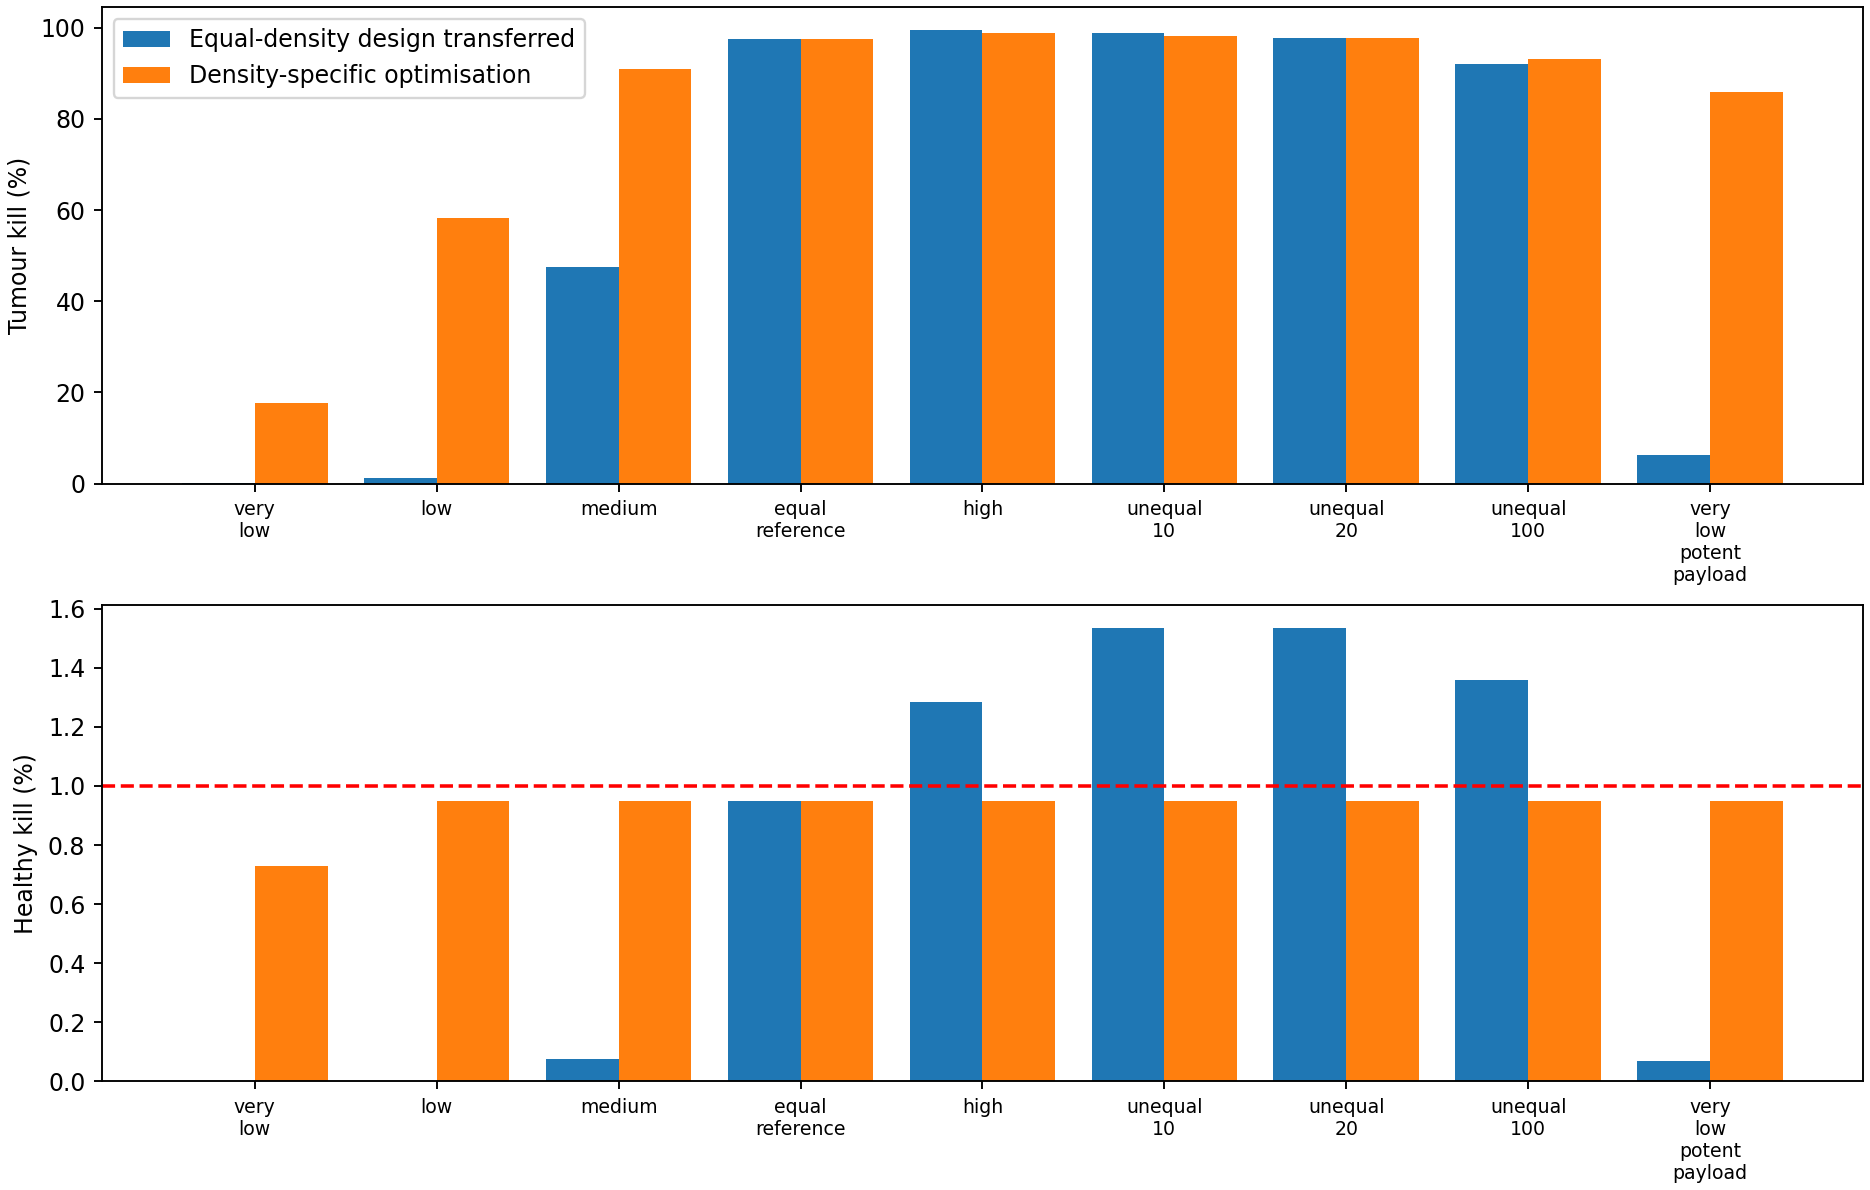
\includegraphics[width=\linewidth]{density_reoptimization_comparison.png}\par
The orange bars use a separately selected set of binding rates at each density pair. They do not imply a single antibody works at every density. The blue bars hold the equal-density design's rates fixed. Raising efficacy by exceeding the healthy constraint is not considered successful optimisation.

\textbf{Search evidence.} Across the nine scenarios, 10582 fresh search/refinement evaluations were performed. Multiple local searches can terminate without a convergence certificate (5 local terminations reported failure). We select verified feasible evaluations, including intermediate ones, rather than treating an optimiser's termination flag as proof of optimality. Two-seed agreement is reported on the final page. Similar efficacy does not identify unique rates.
\newpage
\section*{Selected smooth time courses}
\par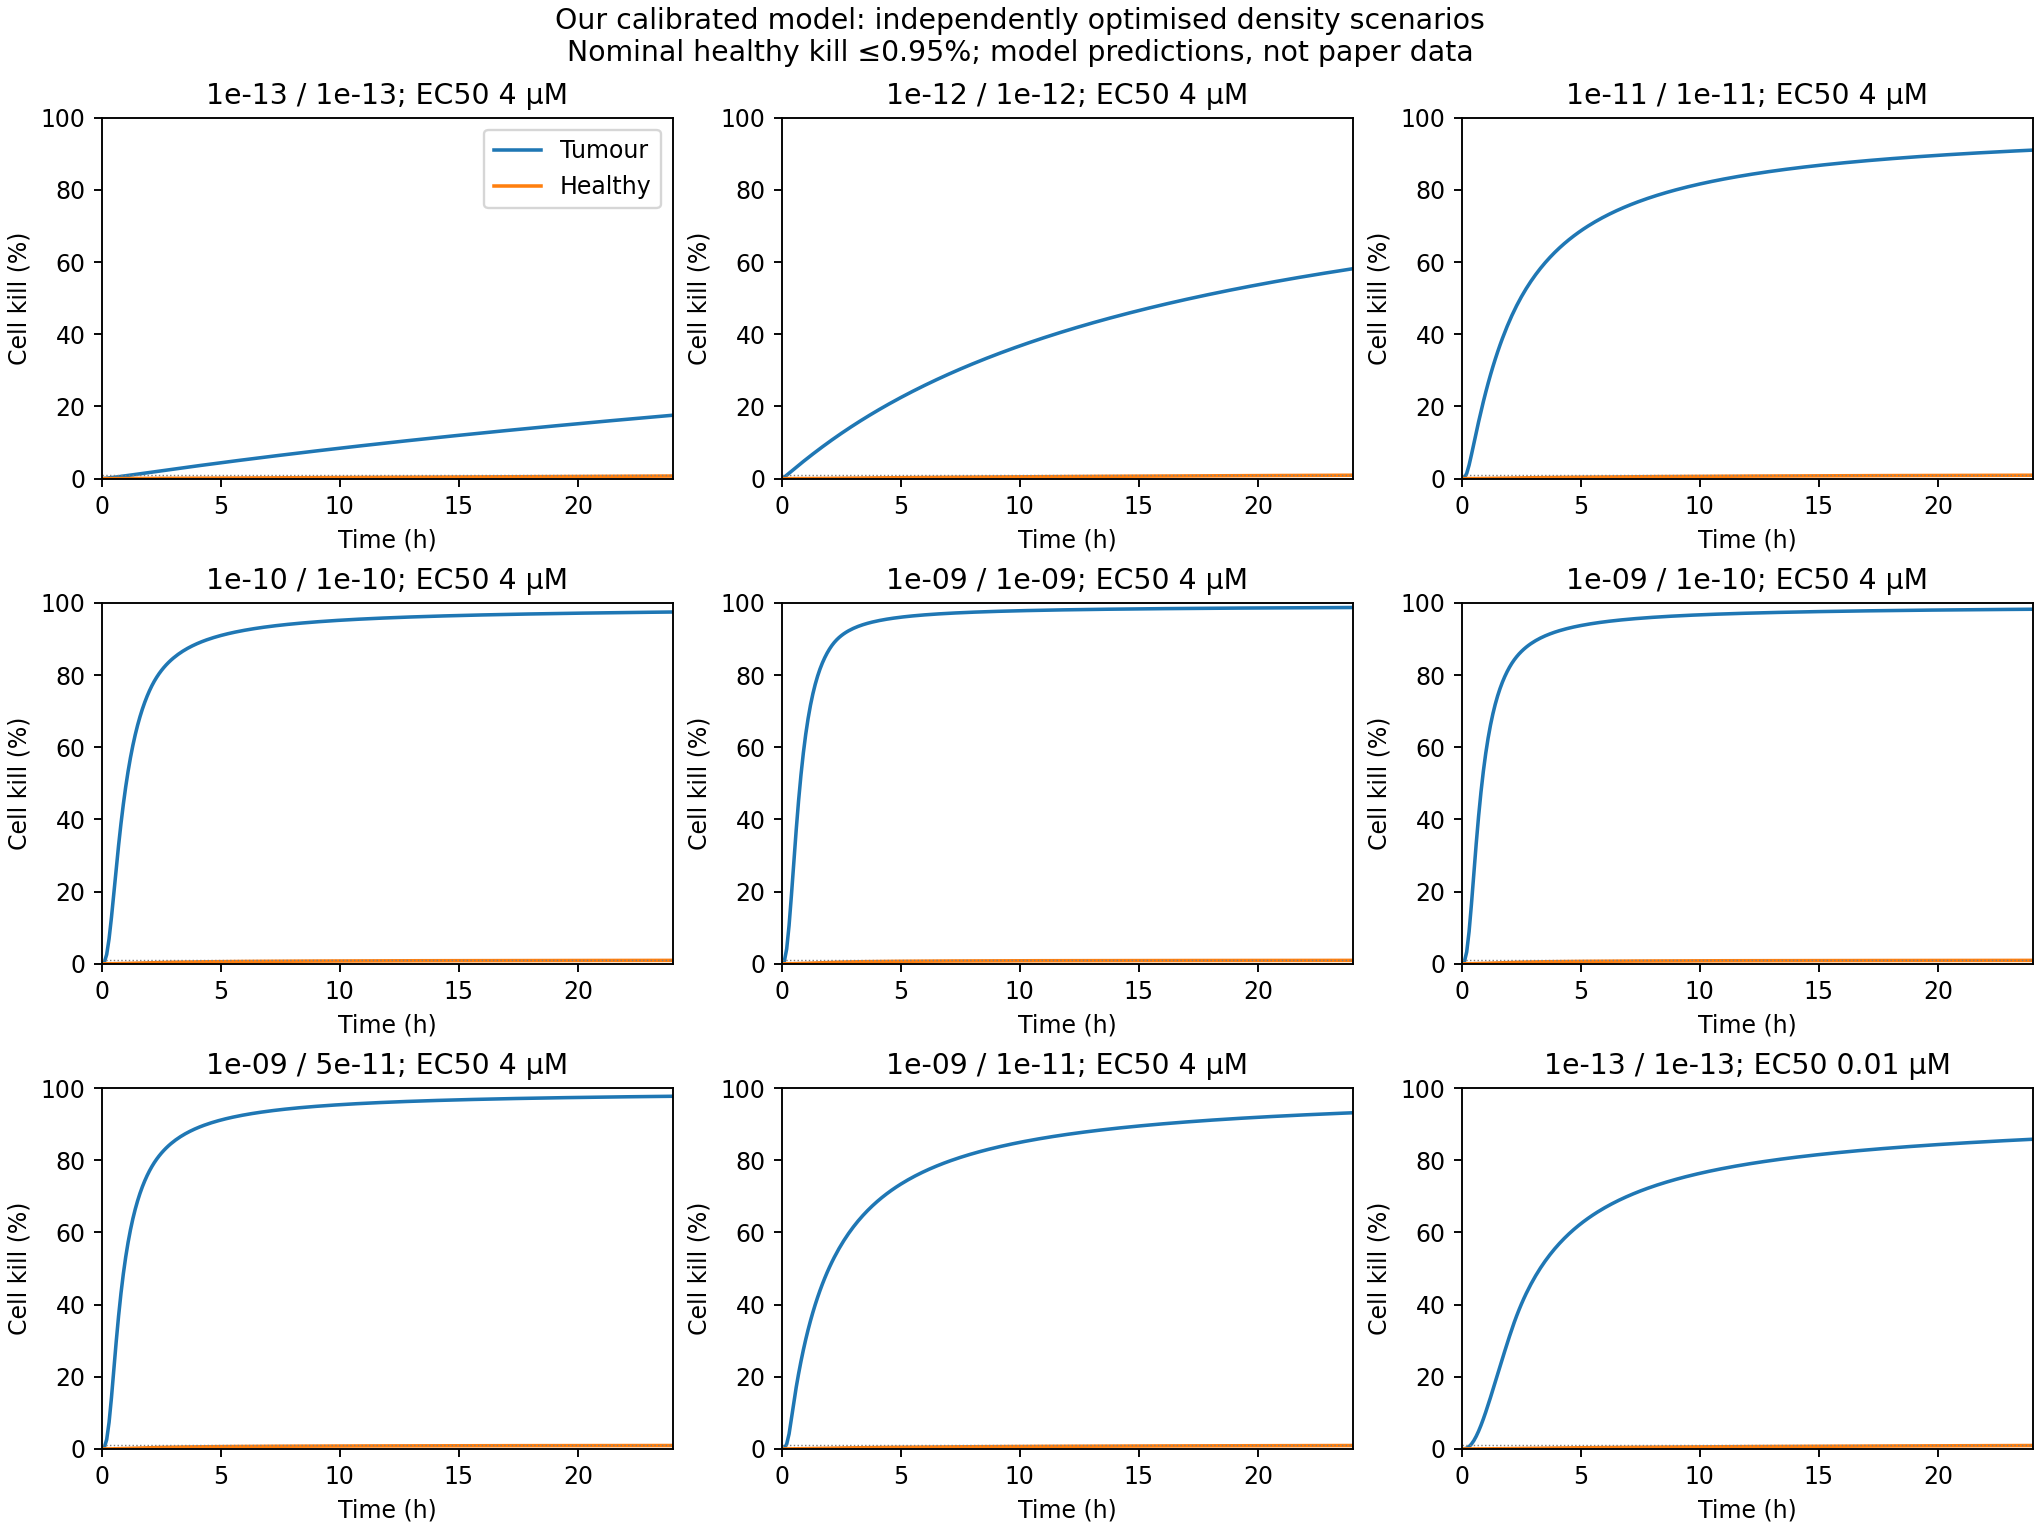
\includegraphics[width=\linewidth]{optimized_timecourses.png}\par
All curves are direct ODE trajectories for selected designs at tight tolerances. They are not scatter-search points, smoothed observations or paper traces. At very low density, efficacy with the 4 $\mu$M payload remains limited. The final panel uses the separately labelled 10 nM payload. Relative to the original equal-density 4 $\mu$M design, the final scenario changes both kinetics and potency. Within that final row, the transferred and reoptimised candidates both use the same 10 nM payload.

\textbf{Reproduction of published candidates remains incomplete.} Under our new model, the published binding rates produce:
\begin{center}\small\begin{tabular}{lrrrr}\toprule
Candidate & Uptake ($\mu$M) & T2 RO (\%) & Tumour kill (\%) & Healthy kill (\%)\\\midrule
figure4\_bispecific & 56 & 0.0207 & 93.3 & 15 \\
figure6 & 280 & 36.4 & 98.6 & 1.8 \\
figure8 & 277 & 91.8 & 98.6 & 4.66 \\
\bottomrule\end{tabular}\end{center}
The first two uptake endpoints were calibration targets; agreement there is expected. The paper's Figure 8 uptake (approximately 240 $\mu$M) and final T2 occupancy (approximately 66\%) are visual estimates withheld from fitting. A mismatch here is retained honestly. Finding selective designs in our model does not validate the paper's exact optimum or the physiological calibration.
\newpage
\section*{Verification, sensitivity and practical limits}
\textbf{Numerical verification.} Every selected candidate was reintegrated with BDF and Radau at relative tolerance $10^{-9}$ and absolute tolerance $10^{-12}$. Maximum endpoint disagreement: 1.14e-09 (kill fraction). Maximum relative mass-balance error: 6.38e-13. Maximum target-label exchange error: 2.22e-16. All selected trajectories remain below 1\% nominal healthy kill. The model unit tests also cover no-dose/no-target limits, occupancy, receptor accounting and nonlinear healthy-population weighting.

\textbf{Sensitivity with rates held fixed.} We independently perturb accessible cell burden, effective intracellular volume and turnover by $\pm20\%$; set background clearance to zero or double; and restore the original Sengers off-rate convention. These are one-at-a-time diagnostic scenarios, not a probability distribution or a clinical confidence interval. No reoptimisation is performed for these perturbations.
\begin{center}\small\begin{tabular}{crr}\toprule
ID & Two-seed tumour spread (percentage points) & Maximum perturbed healthy kill (\%)\\\midrule
1 & 0.0002 & 0.901 \\
2 & 0.0000 & 1.161 \\
3 & 0.0000 & 1.068 \\
4 & 0.0000 & 1.016 \\
5 & 0.0000 & 1.011 \\
6 & 0.0000 & 1.004 \\
7 & 0.0000 & 1.000 \\
8 & 0.0000 & 1.034 \\
9 & 0.0001 & 1.171 \\
\bottomrule\end{tabular}\end{center}
Any perturbed healthy kill above 1\% means the selected design is not robust to that tested model uncertainty. The 0.95\% nominal limit should not be interpreted as a robust safety guarantee. A robust-design extension would optimise against the worst case across a prespecified uncertainty set, rather than reinterpret these nominal results.

\textbf{Interpretation.} The model supports exploring how affinity, kinetic timescales, avidity, expression density and potency jointly determine selectivity. It provides reproducible candidate designs and exposes when low density limits efficacy. It does not establish a unique biological optimum, exact paper reproduction, sequence-level feasibility or clinical safety. Boundary rates and physiological uncertainty should guide future model and experimental work.

\textbf{Reproduce.} Run \texttt{python replication/final\_density\_optimization.py --workers 4}, followed by \texttt{python replication/report\_final\_density.py}. Use \texttt{--resume} to reuse completed scenario searches from this configuration. Configuration JSON, per-seed evaluation CSVs, unrounded selected rates, all time courses, sensitivity tables, verification results and this LaTeX source accompany the PDF.
\end{document}
